\subsection*{Общая характеристика работы}

\newcommand{\actuality}{\underline{\textbf{Актуальность темы.}}}
\newcommand{\aim}{\underline{\textbf{Целью}}}
\newcommand{\tasks}{\underline{\textbf{задачи}}}
\newcommand{\scope}{\underline{\textbf{Область исследования}}}
\newcommand{\subject}{\underline{\textbf{Предметом исследования}}}

\newcommand{\defpositions}{\underline{\textbf{Основные положения, выносимые на~защиту:}}}
\newcommand{\novelty}{\underline{\textbf{Научная новизна:}}}
\newcommand{\influence}{\underline{\textbf{Практическая значимость}}}
\newcommand{\reliability}{\underline{\textbf{Достоверность}}}
\newcommand{\probation}{\underline{\textbf{Апробация работы.}}}
\newcommand{\contribution}{\underline{\textbf{Личный вклад.}}}
\newcommand{\publications}{\underline{\textbf{Публикации.}}}


{\aim} работы является разработка интеллектуальной системы повышения эффективности деятельности ИТ-службы предприятия. \par
{\scope}~--- разработка методов и алгоритмов решения задач системного анализа, оптимизации, управления, принятия решений и обработки информации в ИТ-отрасли.\par
{\subject}  является процесс регистрации и устранения проблемных ситуаций, возникающих в ИТ-инфраструктуре предприятия.\par

Для достижения поставленной цели необходимо было решить следующие {\tasks}:
\begin{enumerate}
  \item Провести теоретико-множественный и теоретико-информационный анализ сложных систем в области поддержки информационной инфраструктуры;
  \item Создать модель целевой области;
  \item Исследовать модели мышления и выбрать наиболее подходящую;
  \item На основе выбранной модели мышления разработать модель проблемно-ориентированной системы управления, принятия решений и оптимизации процесса принятия, анализа и обработки запросов пользователя в области обслуживания информационной структуры предприятия;
  \item Создать архитектуру приложения на основе модели;
  \item Реализовать на основе этой архитектуры прототип интеллектуальной вопросно-ответной системы повышения эффективности деятельности ИТ-службы предприятия;
  \item Провести апробацию прототипа на тестовых данных.
\end{enumerate}

\defpositions
\begin{enumerate}
  \item Теоретико-множественный и теоретико-информационный анализ сложных систем в области поддержки информационной инфраструктуры;
  \item Построенная модель проблемно-ориентированной системы управления, принятия решений и оптимизации технических объектов в области обслуживания информационной инфраструктуры;
  \item Созданный прототип программной реализации модели проблемно-ориентированной системы управления, принятия решений и оптимизации обработки запросов пользователя в области обслуживания информационной инфраструктуры;
  \item Апробация прототипа проблемно-ориентированной системы управления, принятия решений и оптимизации деятельности на контрольных примерах и анализ ее результатов.
\end{enumerate}

\novelty проведенного исследования состоит в следующем:
\begin{enumerate}
  \item Создана модель проблемно-ориентированной системы управления, принятия решений в области обслуживания информационной структуры предприятия на основе модели мышления;
  \item Представлены новая модель данных для модели мышления и оригинальный способ хранения для этой модели, эффективный по сравнению с другими базами данных;
  \item Выполнено оригинальное исследование моделей мышления применительно к области обслуживания информационной структуры предприятия;
  \item На основе модели мышления Мински созданы архитектура системы обслуживания информационной структуры предприятия и программный прототип этой системы.
\end{enumerate}

\influence\ 
Система, разработанная в рамках данной диссертации носит значимый практический характер. Идея работы зародилась под влиянием производственных проблем в ИТ-отрасли, с которыми автор сталкивался каждый день в процессе разрешения различных инцидентов, возникающих в деятельности службы технической поддержки \icl~--- одном из крупнейших системообразующих предприятий ИТ-области Республике Татарстан. Поэтому было необходимо выработать глубокое понимание конкретной предметной области, чтобы выбрать приемлемое решение, получившее практическое применение в работе на проекте поддержки крупной сети продуктовых магазинов. \par
\reliability\ научных исследований и практических рекомендаций
базируется на корректной постановке общих и частных рассматриваемых задач,  использовании известных фундаментальных теоретических положений системного анализа, достаточном объёме данных, использованных при статистическом моделировании, и широком экспериментальном материале, использованном для численных оценок достижимых качественных показателей. \par 
Исследования, проведенные в диссертации, соответствуют паспорту специальности 05.13.01~--- Системный анализ, управление и обработка информации, сопоставление приведено в таблице \ref{ResearchDescription}.

\begin{longtable}{|p{7cm}|p{9cm}|}
 \caption[Сопоставление направлений исследований в рамках специальности 05.13.01 и исследований, проведенных в диссертации]{Сопоставление направлений исследований в рамках специальности 05.13.01 и исследований, проведенных в диссертации}\label{ResearchDescription} \\ 
 \hline
 
 \multicolumn{1}{|c|}{\textbf{Направление исследования}} & \multicolumn{1}{c|}{\textbf{Результат работы}}  \\ \hline 
\endfirsthead
\multicolumn{2}{c}%
{{\bfseries \tablename\ \thetable{} -- продолжение}} \\
\hline \multicolumn{1}{|c|}{\textbf{Направление исследования}} &
\multicolumn{1}{c|}{\textbf{Результат работы}}  \\ \hline 
\endhead

\hline \multicolumn{2}{|r|}{{Продолжение следует}} \\ \hline
\endfoot

\hline \hline
\endlastfoot
\hline
   Разработка критериев и моделей описания и оценки эффективности решения задач системного анализа, оптимизации, управления, принятия решений и обработки информации & В рамках работы была разработана модель системы принятия решения и обработки информации в области решения запросов пользователя на естественном языке. \\
   \hline
   Разработка проблемно-ориентированных систем управления, принятия решений и оптимизации технических объектов & По модели, разработанной в предыдущем пункте был разработан прототип системы принятия решения Thinking Understanding, который был испытан на модельных данных.\\
   \hline
   Методы получения, анализа и обработки экспертной информации & В рамках системы TU был разработан метод обработки экспертной информации - обучение при помощи модели мышления TU, основанной на принципах модели 6-ти Марвина Мински. \\
   \hline
   Разработка специального математического и алгоритмического обеспечения систем анализа, оптимизации, управления, принятия решений и обработки информации & В рамках разработки системы TU были созданы специальные алгоритмы для анализа запросов пользователя и принятия решений.\\
  \hline 
  Теоретико-множественный и теоретико-информационный анализ сложных систем & В рамках работы был проведен комплексный анализ области поддержки программного обеспечения, с помощью которого была построена система данной области и выделены участки для оптимизации принятия решений.\\
  \hline
  Методы и алгоритмы интеллектуальной поддержки при принятии управленческих решений в технических системах & Система, разработанная в рамках данной работы в включает в себя инновационные методы и алгоритмы поддержки принятия решений, использующих в своей основе модель мышления на базе модели мышления Человека, описанной в книге Марвина Мински. \\ 
  \hline
  Визуализация, трансформация и анализ информации на основе компьютерных методов обработки информации & Представлена наглядная визуализация данных по системному анализу области удаленной поддержки инфраструктуры. \\
  \hline	
\end{longtable}


\probation\
 Основные результаты диссертационной работы докладывались на следующих конференциях:
\begin{itemize}
	\item Десятая молодежная научная школа-конференция "Лобачевские чтения~---2011. Казань, 31 октября~--4 ноября 2011";
	\item 3rd World Conference on Information Technology (WCIT-2012); 
	\item Искусственный интеллект и естественный язык (AINL-2013);
	\item Электронная Казань~--- 2014;
	\item Электронные библиотеки: перспективные методы и технологии, электронные коллекции (RCDL-2014);
	\item Agents and multi-agent systems: technologies and applications (AMSTA-2015).
\end{itemize}
Практическая апробация результатов работы проводилась на выгрузке инцидентов из системы регистрации запросов службы технической поддержки ИТ-инфраструктуры \icl. Созданная система показала требуемые результаты (процент успешно обработанных запросов более чем 30\%) обработки данной информации.
\contribution\ Автор исследовал целевую область: проводил анализ запросов пользователей и классифицировал их, вместе с Талановым Максимом Олеговичем изучал модель мышления Марвина Мински; создавал базовую архитектуру систему; вместе с Талановым Максимом Олеговичем проводил разработку компонентов модели, адаптируя теорию Марвина Мински. Автор проводил испытание системы на целевых запросах; отлаживал работу системы.
\publications\ Основные результаты по теме диссертации изложены в 9 печатных изданиях  \cite{Lobachevskii},\cite{WCIT-2012},\cite{AINL-2013},\cite{ISGZ}, \cite{IJSE-1}, \cite{IJSE-2}, \cite{RCDL-2014}, \cite{AMSTA-2015}, \cite{VAK-1}, из которых статьи \cite{RCDL-2014},\cite{AMSTA-2015} проиндексированы в БД Scopus, статья \cite{AMSTA-2015} проиндексирована в БД Web Of Science, работа \cite{VAK-1} опубликована в журнале из списка ВАК, статья  \cite{ISGZ} проиндексирована в БД РИНЦ, работы \cite{Lobachevskii},\cite{WCIT-2012},\cite{AINL-2013},\cite{ISGZ} опубликованы в материалах международных и всероссийских конференций.



 % Характеристика работы по структуре во введении и в автореферате не отличается (ГОСТ Р 7.0.11, пункты 5.3.1 и 9.2.1), потому её загружаем из одного и того же внешнего файла, предварительно задав форму выделения некоторым параметрам

%Диссертационная работа была выполнена при поддержке грантов ...

%\underline{\textbf{Объем и структура работы.}} Диссертация состоит из~введения, четырех глав, заключения и~приложения. Полный объем диссертации \textbf{ХХХ}~страниц текста с~\textbf{ХХ}~рисунками и~5~таблицами. Список литературы содержит \textbf{ХХX}~наименование.

%\newpage
\subsection*{Содержание работы}
Во \underline{\textbf{введении}} обосновывается актуальность исследования, проводимых в рамках данной диссертационной работы, дается общая характеристика работы. Проводится обзор области и производится постановка задачи. \par
\underline{\textbf{Первая глава}} посвящена обзору интеллектуальных систем регистрации и анализа проблемных ситуаций, возникающих в ИТ-инфраструктуре предприятия. Здесь представлен сравнительный анализ систем регистрации и устранения проблемных ситуаций. В главе определяются основные требования к интеллектуальным системам регистрации и анализа проблемных ситуаций в ИТ. Одним из важных элементов подобных систем является обработка естественного языка, поэтому здесь представлен сравнительный анализ методов и комплексов обработки текстов на естественном языке. \\
Во время анализа были использованы следующие обработчики естественного языка: Open NLP; Relex; StanfordParser.
Результат работы подсчитывался при помощи метрик, представленных в Таблице \ref{Metrics}. 

\begin{table} [htbp]
  \centering
  \parbox{15cm}{\caption{Таблица метрик}\label{Metrics}}
%  \begin{center}
  \begin{tabular}{| p{5cm} |p{5cm}| p{5cm} |}
  \hline

\textbf{Метрика} & \textbf{Описание} & \textbf{Формула} \\
  \hline

Precision	& Точность & 
$$ 
P=\frac{tp}{tp+fp}
$$ где P~--- precision, tp~---  успешно обработанные, fp~--- ложно успешные \\
 \hline
Recall	& Чувствительность & 
$$ 
R=\frac{tp}{tp+fn}
$$ где R~--- recall, tp~--- успешно обработанные, fn~--- ложно неуспешные \\
 \hline
F	& F~--- measure (результативность) & 
$$ 
F=\frac{P*R}{P+R}
$$ Где P~--- precision, R~--- recall.   \\
 \hline
  \end{tabular}
%  \end{center}
\end{table}

Результаты приведены на сводной диаграмме Рисунок \ref{img:ParserComp}. \\
Все рассмотренные системы не соответствуют полному комплексу необходимых требований. В Таблице \ref{Comparsion} приведены сводные данные по системам.  Ввиду развитости и доступности было решено использовать OpenCog RelEx.

\begin{longtable}{|p{6cm}|p{0.5cm}|p{0.5cm}|p{0.5cm}|}
 \caption[Сравнительный анализ существующих решений]{Сравнительный анализ существующих решений}\label{Comparsion} \\ 
 \hline
 
 \multicolumn{1}{|c|}{\textbf{Сравнительный пункт}} & \multicolumn{1}{c|}{\textbf{HP Open View}} & \multicolumn{1}{c|}{\textbf{ServiceNOW}} & \multicolumn{1}{c|}{\textbf{IBM Watson}} \\ \hline 
\endfirsthead
\multicolumn{2}{c}%
{{\bfseries \tablename\ \thetable{} -- продолжение}} \\
\hline \multicolumn{1}{|c|}{\textbf{Сравнительный пункт}} & \multicolumn{1}{c|}{\textbf{HP Open View}} & \multicolumn{1}{c|}{\textbf{ServiceNOW}} & \multicolumn{1}{c|}{\textbf{IBM Watson}}  \\ \hline 
\endhead
\endfoot

\hline \hline
\endlastfoot
\hline
   Мониторинг & Да & Да & Да \\
   \hline
   Регистрация инцидентов & Да & Да & Да\\
   \hline
   Управление системами & Да & Нет & Нет \\
   \hline 
   Создание цепи обработки (Workflow) инцидента & Да & Да & Нет \\
   \hline 
   Понимания и формализацию запросов на естественном языке & Нет & Нет & Да \\
   \hline 
   Поиск решений & Нет & Нет & Да \\
   \hline 
   Применение решений & Нет & Нет & Нет \\
   \hline
   Обучение решению инцидента & Нет & Нет & Да \\
   \hline
   Умение проводить логические рассуждения: генерализацию, специализацию, синонимичный поиск & Нет & Нет & Нет \\
   \hline
   
\end{longtable}
%=================
%===Second chapter
%=================

\underline{\textbf{Вторая глава}} посвящена построению модели интеллектуальной системы принятия решений для регистрации и анализа проблемных ситуаций в ИТ-инфраструктуре предприятия.
Созданными и испытанными моделями, использованными при создании системы принятия решений для регистрации и анализа проблемных ситуаций в ИТ-инфраструктуре предприятия, являются:
 \begin{itemize}
	\item модель Menta 0.1, построенная с использованием деревьев принятия решений;
	\item модель Menta 0.3, построенная с использованием генетических алгоритмов;
	\item модель TU 1.0, основанная на модели мышления Марвина Мински.
\end{itemize} \par

Модель, построенная на базе нейронных сетей (поддерживающая обучение) была отброшена на предварительной стадии оценки, так как она предъявляет большие требования к производительности, что в свою очередь порождает высокую стоимость. Далее каждая модель будет рассмотрена подробно.

\textbf{Модель с использованием Деревьев Принятия Решений (Menta 0.1)}.
Данная модель являлась одной из первых, которая была опробована. Модель была основана на деревьях принятия решений. В построение модели данной системы использовались следующие компоненты: обработка запросов на естественном языке; поиск решения; применение решения. \par
Системы была ориентирована на выполнение простых команд, например, добавить поле на форму. В целом работа системы описывается следующим алгоритмом:
\begin{enumerate}
	\item Получение и формализация запроса
	\item Поиск решения при помощи Деревьев Принятия Решений
	\item Изменение модели приложения в формате OWL
	\item Генерация и компиляция приложения
\end{enumerate} \par
После проведения экспериментов были выявлены следующие проблемы: отсутствие устойчивости к ошибкам входной информации: грамматическим и содержательным. Например, входной файл не имел отношения к программной системе, модель которой была в базе знаний в формате OWL; система поиска решения работала только в рамках модели одной программы;  отсутствовала функция обучения. \par



\textbf{Модель с использованием Генетических алгоритмов на базе модели мышления Питера Норвига (Menta 0.2-0.3)}.
В рамках модели Menta 0.3 были отработаны следующие основные компоненты будущей итоговой модели: критерии приемки (Acceptance Criteria); How-To~--- для хранения решений проанализированных проблем; формат данных OWL; использование логических вычислений для проверки решения. Система Menta 0.3 содержала внутри себя модель целевого приложения (как и Menta 0.1) и список решений тех или иных проблем (How-To). При помощи генетического алгоритма модель строила How-To решение проверяла его при помощи логического движка NARS на соответствие входным критериям приемки. С точки зрения генетических алгоритмов это~--- функция отбора особей из поколения. \par
После проведения экспериментов были выявлены следующие проблемы: отсутсвие обучения; отсутсвие обработки естественного языка; после апробации оказалось, что критерии приемки практически описывают необходимое решение (то которое должно быть найдено), что являлось недопустимым. \par


\textbf{Модель мышления Марвина Мински (Модель 6-ти)}.
Модель была построена с применением теории Марвина Мински. Эта модель сохранила следующие основные концептуальные элементы предыдущих моделей и показала свою состоятельность на контрольных примерах: Acceptance Criteria; обучение; поиск и применение решения; Отсутсвие обработки естественного языка. Данная модель является более универсальной и представляет собой верхнеуровневую архитектуру обработки запроса (мышления), где компонентами являются лучшие части предыдущих систем. Реализация модели получила название TU. \par
Одним из основных компонентов системы является
\underline{\triplet}. На Рисунке \ref{img:csw} представлена схематичное изображение Критика-Селектора-Образа мышления. \\
\begin{figure} [h] 
  \center
  \includegraphics [scale=1.0] {CSW}
  \caption{Критик-Селектор-Образ мышления} 
  \label{img:csw}  
\end{figure}


\underline{Критик (Critic)} представляет собой определенный переключатель: внешние обстоятельства, события или иное воздействие. Например, «включился свет, и зрачки сузились», «обожглись и одернули руку». Критик активируется только тогда, когда для этого достаточно обстоятельств. Одновременно могут активироваться несколько критиков. Например, человек решает сложную задачу, идет активация множество критиков: выполнить расчет, уточнить технические детали. Кроме того, параллельно может активироваться критик переработки, сообщающий о необходимости отдыха.\par
\underline{Селектор (Selector)} занимается выбором определенных ресурсов, которыми также являются Образ мышления. \par
\underline{Образ мышления (WayToThink)}~--- это способ решения проблемы. Образ мышления может быть сложным и, например, активировать другие критики. Например,  размышляя над проблемой, специалист понимает, что нужно произвести полный перебор, и тут он решает поискать готовое решение: а может кто-то уже сделал такой перебор и можно будет его использовать. Здесь "поиск готового решения" является критиком внутри образа мышления "поиск решения".\par

На рисунке \ref{img:csw_ex} представлена расширенная модель работы триплета \triplet. Критик активирует Селектор, который активирует Образ мышления (синий круг). Последний в свою очередь может активировать нового Критика или же совершить определенные действия. Например, зажегся зеленый свет светофора, значит, можно переходить дорогу. Под ресурсами здесь понимается набор знаний из базы знаний: Критики, Селекторы, Образы мышления, готовые решения. \par
Если активировалось много критиков, то проблему нужно уточнить, так как степень неопределенности слишком высока. Если проблема очень похожа на уже проанализированную, то можно действовать и судить по аналогии. \par
\begin{figure} [h] 
  \center
  \includegraphics [scale=1.0] {CSW_EX}
  \caption{Критик-Селектор-Образ мышления в разрезе ресурсов} 
  \label{img:csw_ex}  
\end{figure}
Другой важной концепцией теории являются уровни мышления. Это концепция распределяет активность мышления между 6-ю уровнями: чем выше уровень, тем сильне активность. В Таблице \ref{ThinkingLevelDescription} представлено описание уровней мышления с примерами. \par
На этом исследование моделей мышлений было завершено и были сделаны выводы. 
\begin{table} [htbp]
  \centering
  \parbox{15cm}{\caption{Описание уровней мышления модели 6-ти}\label{ThinkingLevelDescription}}
%  \begin{center}
  \begin{tabular}{| p{5cm} | p{11cm} |}
  
  \hline
\textbf{Уровень} & \textbf{Описание} \\
  \hline
  
Инстинктивный уровень	& На данном уровне происходят инстинктивные реакции (врожденные). Например, коленный рефлекс. Общую формулу для этого уровня можно выразить как "Если ..., то сделать так". \\
  \hline

Уровень обученных реакций  & На  данном уровне происходит мышление обученных реакций, то есть тех реакций, которыми человек обучается в течение жизни. Например, переходить дорогу на зеленых свет. Общую формулу для этого уровня можно выразить как "Если ..., то сделать так". \\
  \hline

Уровень рассуждений & а  данной уровне происходит мышление с использованием рассуждений. Если я сделаю так, то будет ... Например, если перебежать дорогу на зеленый свет, то можно успеть вовремя. На данном уровне сравниваются последствия нескольких решений и выбирается оптимальное. Общую формулу для этого уровня можно выразить как "Если ..., то сделать так, тогда будет так". \\
  \hline

Рефлексивный уровень  & На данном уровне происходит рассуждение с учетом анализа прошлых событий. Например, в прошлый раз я побежал на моргающий зеленый и чуть не попал под машину. \\

  \hline
  Саморефлексивный уровень & На данном уровне происходит оценка себя. Строится определенная модель с помощью которой идет оценка своих поступков. Например, мое решение не пойти на это собрание было неверным, так как я упустил столько возможностей, я был легкомысленный. \\
  \hline
  Самосознательный уровень & На данном уровне идет оценка поступков человека с точки зрения высших идеалов и внешних оценок. Например, а что подумают мои друзья? А как бы поступил мой герой? \\
  \hline
  
  \end{tabular}
%  \end{center}
\end{table}


Для программной экспертной системы очень важно обладать способностью мыслить и рассуждать. Например, очень важно  для системы уметь действовать по аналогии. Так как множество запросов типичны и отличаются лишь параметрами. Например, пожалуйста, установить Office, Antivirus и т.д. \par
Также для экспертной системы важно уметь абстрагировать специализированные рецепты решения. К примеру, система научилась решать инцидент "Please install Firefox". Абстрагировав данный инцидент до степени "Please install browser" система сможет теми же способами попробовать решить новый инцидент.\par
После рассмотрения нескольких моделей была выбрана модель мышления Марвина Мински, так как данная модель наиболее точно ложится на целевую область решения инцидентов в области IT. На основе подхода Мински была построена модель системы, которая поддерживает основные функции: обучение, понимание инцидента, поиск решения, применение решения. 


%=================
%===3rd chapter
%=================
В \underline{\textbf{третьей главе}} приведено описание архитектуры и реализации системы, основанной на модели TU.
Архитектура системы представляет собой модули. Основными компоненты системы описаны в Таблице \ref{MainComponents}. Система может функционировать в режиме обучения и в режиме решения запросов. 
\begin{longtable}{|p{7cm}|p{8cm}|}
 \caption[Основные компоненты системы ThinkingUnderstanding]{Основные компоненты системы ThinkingUnderstanding}\label{MainComponents} \\ 
 \hline
 
 \multicolumn{1}{|c|}{\textbf{Компонент}} & \multicolumn{1}{c|}{\textbf{Описание}}  \\ \hline 
\endfirsthead
\multicolumn{2}{c}%
{{\bfseries \tablename\ \thetable{} -- продолжение}} \\
\hline \multicolumn{1}{|c|}{\textbf{Компонент}} &
\multicolumn{1}{c|}{\textbf{Описание}}  \\ \hline 
\endhead

\endfoot

\hline \hline
\endlastfoot
\hline
   TU Webservice & Основной компонент взаимодействия со внешними система, включая пользователя. \\
   \hline
   CoreService & Ядро системы, содержит основные классы.\\
   \hline
   DataService & Компонент работы с данными. \\
   \hline 
   Reasoner & Компонент вероятностной логики. \\
   \hline 
   ClientAgent & Компонент выполнения скриптов на целевой машине. \\
   \hline 
   MessageBus & Шина данных для системы. \\
   \hline 
\end{longtable}
В главе приводится основной рабочий поток работы приложения.
 \begin{enumerate}
	\item Поступает запрос от пользователя \\
	User had received wrong application.
User has ordered Wordfinder Business Economical.
However she received wrong version, she received Wordfinder Tehcnical instead of Business Economical. Please assist.
	\item GoalManger устанавливает цель системы HelpUser
	\item Активируется набор Critic, привязанный к данной цели
	\item PreliminaryAnnorator разбирает фразу
	\item KnowledgeBaseAnnotator создает семантическую сеть и ссылки на нее
	\item Critic, привязанный к цели HelpUser на Рефликсивном уровне запускает WayToThink ProblemSolving с целью: ResolveIncident
	\item Critic на Рефликсивном уровне выбирает WayToThink KnowingHow
	\begin{enumerate}
	\item Запускаются параллельно все Critic, которые привязаны к IncidentClassification Critic, который привязан к ResolveIncident цели, в данном случае это DirectInstruction, ProblemWithDesiredState, ProblemWithoutDesiredState
	\item Selector выбирает наиболее вероятный результат работы среди всех результатов компонентов. В данном случае будет результат работы Problem Description with desired state.
	\item KnowingHow сохраняет варианты выбора Selector.
	\item Simulation WayToThink с параметрами "Создать модель текущий ситуации" создает: CurrentSituation, User, Software
	\item Reformulation WayToThink, используя результаты предыдущего шага синтезирует артефакты, которых не хватает, чтобы получить из CurrentState DesiredState, так как он не указан явно. WayToThink запускает Critic размышления, чтобы найти корень проблемы. Он находит CurrentState- Wordfinder Tehcnical, DesiredState-Wordfinder Business Economical
	\item Рефлексивные Critic оценивают состояние системы - на каком шаге она находится, и если цель не достигнута, то запускают другой WayToThink, например, DirectInstruction. 
	\item Critic генерации решения запускает KnowingHow WayToThink, ExtensiveSearch.
	\item Selector выбирает наиболее вероятный образ мышления. В данном случае ExtensiveSearch, который будет находить решения, позволяющие привести систему в необходимое состояние (DesiredState). Если он не сможет, то он иницирует коммуникацию с пользователем. 
 \end{enumerate}
	 \item Рефлексивный Critic проверяет состояние системы. Если Цель достигнута, то пользователю посылается ответ.
	 \item Само Сознательные Critic активируется на данном шаге и сохраняют информацию о затратах на решение.
  \end{enumerate}
В главе приведено описание созданной специально для системы модели данных TUKnowledge \ref{img:KnowledgeClass}.

\begin{figure} [h] 
  \center
  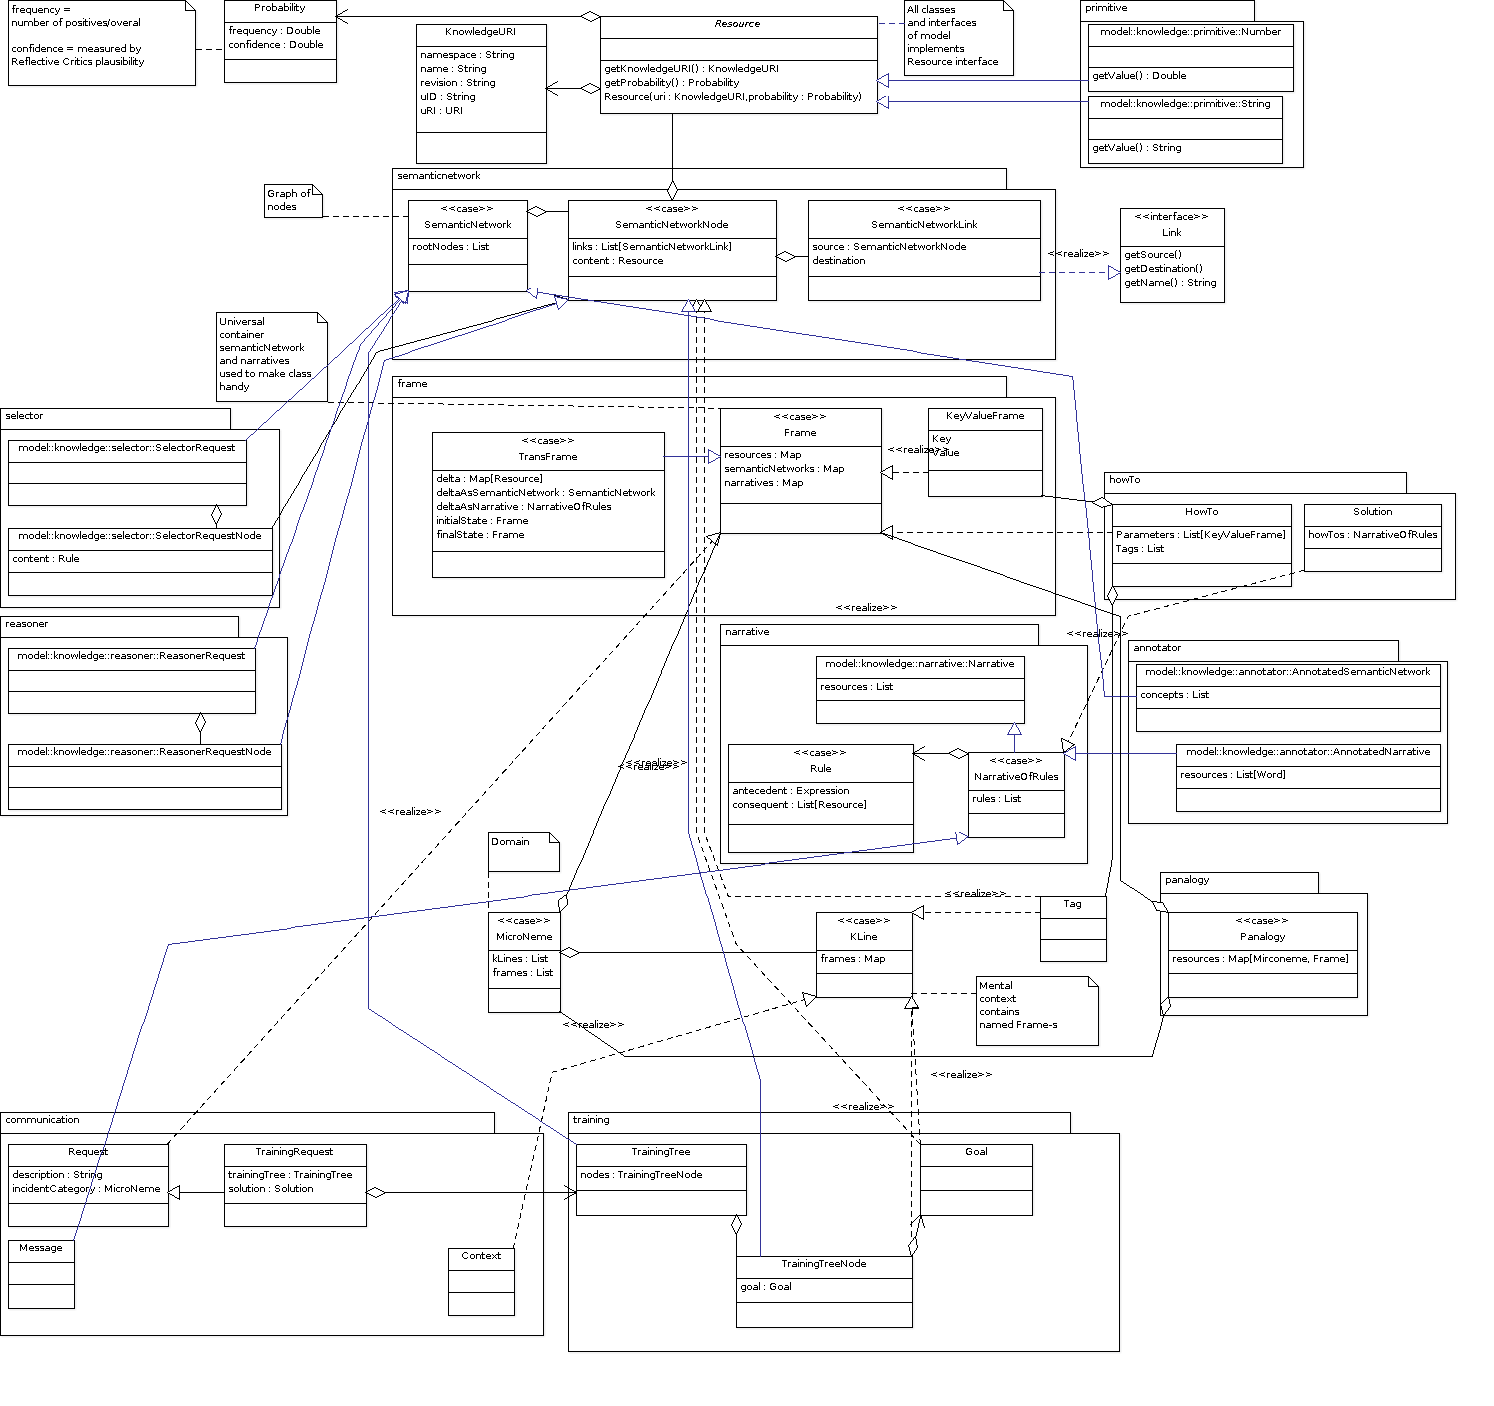
\includegraphics [scale=0.33] {KnowledgeClass}
  \caption{Схема данных TU Knowledge в формате UML} 
  \label{img:KnowledgeClass}  
\end{figure}
\clearpage
%=================
%===4 chapter
%=================
В \underline{\textbf{Главе 4}} приведены Экспериментальные исследования эффективности работы модели TU.
Система показала свою жизнеспособность на модельных данных. Были проведены тесты в сравнении с работой человеческого специалиста. Был выбран контрольный список инцидентов. Сравнивался поиск решения для инцидентов. Основное время при опросе специалиста тратилось на коммуникацию. В Таблице приведены результаты сравнения \ref{HumanComparison}. Тесты были выполнены на машине Intel Core i7 1700 MHz, 8GB RAM, 256 GB SSD, FreeBSD. 
\begin{longtable}{|p{12cm}|p{2cm}|p{2cm}|}
 \caption[Результаты сравнения с работой человеческого специалиста]{Результаты сравнения с работой человеческого специалиста}\label{HumanComparison} \\ 
 \hline
 
 \multicolumn{1}{|c|}{\textbf{Инцидент}} & \multicolumn{1}{c|}{\textbf{TSS1 (.мс)}} & \multicolumn{1}{c|}{\textbf{TU (.мс)}}  \\ \hline 
\endfirsthead
\multicolumn{2}{c}%
{{\bfseries \tablename\ \thetable{} -- продолжение}} \\
\multicolumn{1}{|c|}{\textbf{Инцидент}} & \multicolumn{1}{c|}{\textbf{TSS1 (.мс)}} & \multicolumn{1}{c|}{\textbf{TU (.мс)}}  \\ \hline 
\endhead

\endfoot

\hline \hline
\endlastfoot
\hline
  Tense is kind of concept. & 15000 & 385 \\
  
  \hline
  Please install Firefox.  & 9000 & 859 \\
  \hline
  Browser is an object.   & 20000 & 400 \\
  \hline
  Firefox is a browser.   & 5000 & 659  \\
  \hline
  Install is an action.    & 8000 & 486 \\
  \hline
  User miss Internet Explorer 8.     & 10000 & 10589 \\
  \hline
  User needs document portal update.    & 15000 & 16543 \\
  \hline
  Add new alias Host name on host that alias is wanted to: hrportal.lalala.biz IP adress on host that alias is wanted to: 322.223.333.22 Wanted Alias:    webadviser.lalala.net    & 10000 & 18432  \\ 
  \hline
  Outlook Web Access (CCC) - 403 - Forbidden: Access is denied & 15000 & 10342\\ 
  \hline
  PP2C - Cisco IP communicator. Please see if you can fix the problem with the ip phone, it's stuck on configuring ip + sometimes Server error rejected: Security etc.     & 13000 & 12343 \\ 
   \hline
  \end{longtable}

%=================
%===Conclusion
%=================
В \underline{\textbf{заключении}} приведены основные выводы по работе.
%% Согласно ГОСТ Р 7.0.11-2011:
%% 5.3.3 В заключении диссертации излагают итоги выполненного исследования, рекомендации, перспективы дальнейшей разработки темы.
%% 9.2.3 В заключении автореферата диссертации излагают итоги данного исследования, рекомендации и перспективы дальнейшей разработки темы.

Решены следующие задачи и достигнуты следующие результаты.
\begin{enumerate}
  \item Создана модель проблемно-ориентированной системы управления, принятия решений в области обслуживания информационной структуры предприятия на основе модели мышления;
  \item Представлены новая модель данных для модели мышления и оригинальный способ ее хранения, эффективный по сравнению с другими базами данных;
  \item Выполнено оригинальное исследование моделей мышления в области обслуживания информационной структуры предприятия;
  \item На основе модели созданы архитектура системы и ее прототип; 
  \item Созданы специальные алгоритмы для анализа запросов пользователей и принятия решений;
  \item Система, разработанная в рамках данной работы, включает в себя инновационные методы и алгоритмы поддержки принятия решений, использует модель мышления на базе модели мышления Мински;
  \item Представлена наглядная визуализация структуры области удаленной поддержки инфраструктуры.
\end{enumerate}

Представленные в диссертации модель мышления, ее архитектура и реализация являются уникальными~--- на данный момент времени это единственная реализация модели мышления Мински. \par
Система, разработанная в диссертации, не является узкоспециализированной. Она также подходит для других областей, где требуется поддержка принятия решений. Например, при постановке медицинского диагноза, чтобы отбросить ложные диагнозы. \par
Кроме того, в систему можно загрузить данные о взаимосвязи органов человека и болезней. Далее, к каждому заболеванию добавить симптом и способ лечения, после этого можно делать запрос с симптомами, и система выдаст список вероятных заболеваний со способами их лечения. \par
В области диагностики проблем можно обучить систему узлам автомобиля, проблемам, с ними связанными, признаками этих проблем и способами их устранения. 





 

%\newpage
\renewcommand{\refname}{\large Публикации автора по теме диссертации}

%\insertbiblioauthor                          % Подключаем Bib-базы
\insertbiblioall

